% TODO
% \subsection{Measuring spiking patterns across the network}

% -Mark certain neurons as recording
% -This can be done as a boolean flag on the neuron to tell it to keep a time
% trace of its potential, or by inserting measurement objects into the simulation.
% These measurement objects can take the form of 

\section{Comparing spiking patterns between two networks.}
\label{Comparingspikingpatternsbetweentwonetworks}

\subsection{Hamming distance}
Due to the descritization of time required in clock based simulation, spikes at
each neuron are aligned to a "grid" of sorts. Therefore, given two binary
vectors holding the spiking state of two neurons, $S_{arr}$ and $S^\prime_{arr}$, the bit at a given index $i$ represents
the spike state at the same discrete point in simulation time in either vector.
With this in mind, it is therefore possible to calculate the number of bits
that must be flipped in $V_{arr}$ for it to contain the same sequence of bits as
$V^\prime_{arr}$. The resulting number is the Hamming Distance. While the
Hamming distance can be used to observe the change in spiking pattern between
two neurons, it is limited as it does not provide a spatial metric of change
between two sequences. Another limitation is derived from its simplicity, as
spiking patterns tell us little about the membrane potential of a neuron leading
up to a spike.

\subsection{Kullback-Leibler divergence}

Where the Hamming Distance provides a method by which binary spiking trains of a
neuron can be compared, Kullback-Leibler (KL) divergence provides a similar
method of comparison for the distribution of potential over time between two
neurons. Comparing potential does have a caveat however: if the total integrated
sum of potential is different between the two neurons, the KL divergence is not
a true measure of comparison. This can be mitigated by running the same
experiment multiple times, while experiment variables are changed in a
probabilistic manner. The average divergence could then be calculated. KL
divergence shares a major caveat with Hamming Distance in that it does not
measure distance. This is best illustrated by figure
\ref{fig:distributioncompKLEMD}, where the large change in distance between
distributions within the sub-figures has no effect on the KL divergence. Also of
note is that divergence is not a symmetrical metric, so $KL(A, B) \neq KL(B,
A)$, so any comparisons of KL divergence must ensure that the same divergence is
being compared.

\begin{figure}[h!]
    \begin{subfigure}{.5\textwidth}
        \centering
        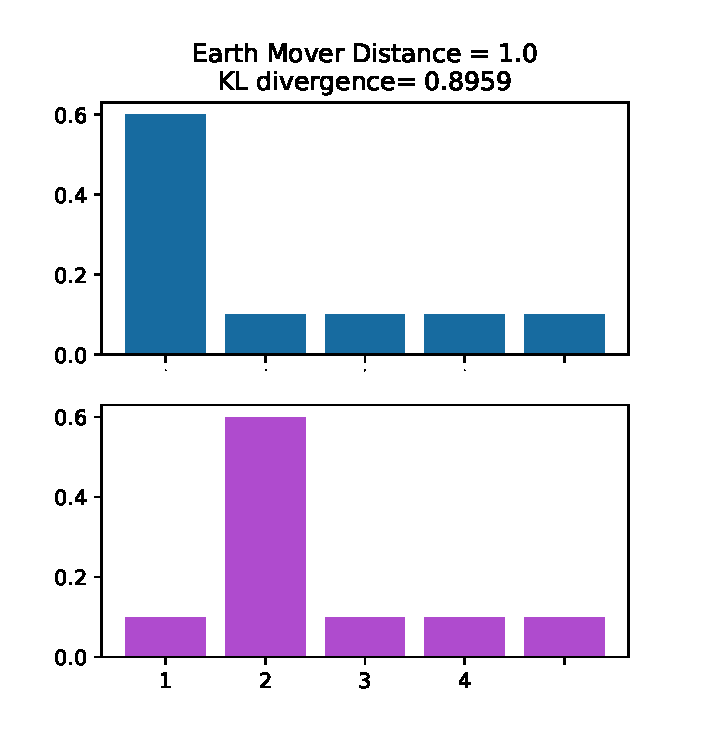
\includegraphics[width=1.0\linewidth]{figures/graphs/EMDvsKLclose.eps}
        \caption{Close distributions}
        \label{fig:closedist}
    \end{subfigure}%
    \begin{subfigure}{.5\textwidth}
        \centering
        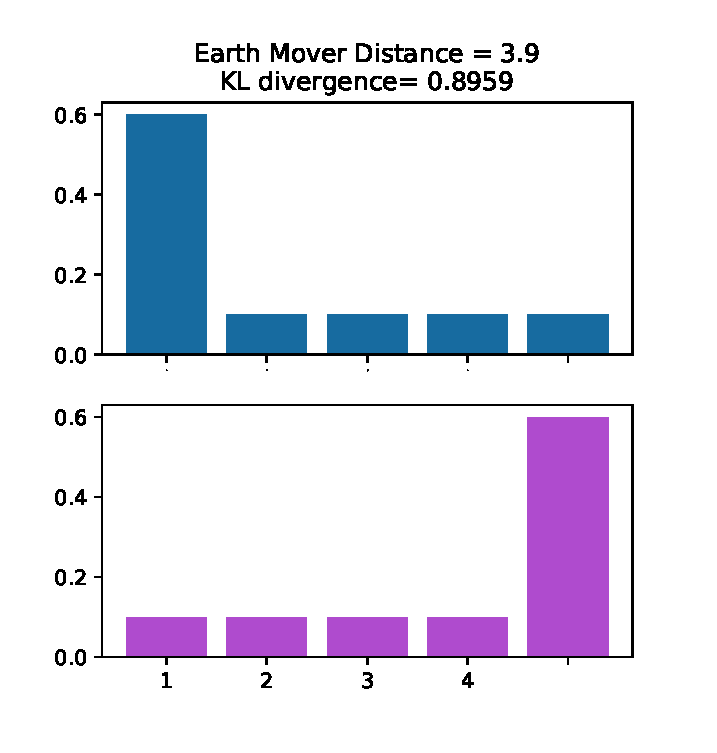
\includegraphics[width=1.0\linewidth]{figures/graphs/EMDvsKLfar.eps}
        \caption{Distant distributions}
        \label{fig:fardist}
    \end{subfigure}
    \caption[Comparison between Earth Mover's Distance and Kullback-Leibler Divergence]{Comparison between Earth Mover's Distance and Kullback-Leibler Divergence on two pairs of distributions with the same integral (area). The closeness of the distributions is reflected in a lower EMD while KL divergence remains the same. EMD is therefore a more intuitive metric to compare distributions.}
    \label{fig:distributioncompKLEMD}
\end{figure}

\FloatBarrier

\subsection{Earth Mover's Distance (EMD)}

Also known as the `Wasserstein Distance', Earth Mover's Distance is, simply put,
given two different mounds of earth, the amount of earth that would need to be
moved from one to the other such that both mounds are the same. More formally,
given two distributions in N-dimensional space $P, Q$, the Earth Mover's
Distance is the N-dimensional distance between them \autocite{pele_fast_2009}. While more computationally
expensive to calculate than Kullback-Leibler divergence, EMD is symmetric, and
more importantly, is aware of relative space between data-points when comparing
distributions. This comparison is shown in figure
\ref{fig:distributioncompKLEMD}, where a change in distribution distance between
the two sub-figures changes the total EMD between them.